\documentclass[12pt,prb,aps,epsf]{report}
\usepackage[utf8]{inputenc}
\usepackage{amsmath}
\usepackage{amsfonts}
\usepackage{amssymb}
\usepackage{graphicx} 
\usepackage{latexsym} 
\usepackage[toc,page]{appendix}
\usepackage{listings}
\usepackage{xcolor}
\usepackage{soul}
\usepackage[T1]{fontenc}
\usepackage{amsthm}
\usepackage{mathtools}
\usepackage{setspace}
\usepackage{array,multirow,makecell}
\usepackage{geometry}
\usepackage{textcomp}
\usepackage{float}
%\usepackage{siunitx}
\usepackage{cancel}
%\usepackage{tikz}
%\usetikzlibrary{calc, shapes, backgrounds, arrows, decorations.pathmorphing, positioning, fit, petri, tikzmark}
\usepackage{here}
\usepackage{titlesec}
%\usepackage{bm}
\usepackage{bbold}

\geometry{hmargin=2cm,vmargin=2cm}

\begin{document}
	
	\title{MP 10 Spectrométrie optique}
	\author{Etienne}
	
	\maketitle
	
	\tableofcontents
	
	\pagebreak
	
\subsection{Introduction}

\section{Spectromètre USB}

\begin{figure}
	\centerline{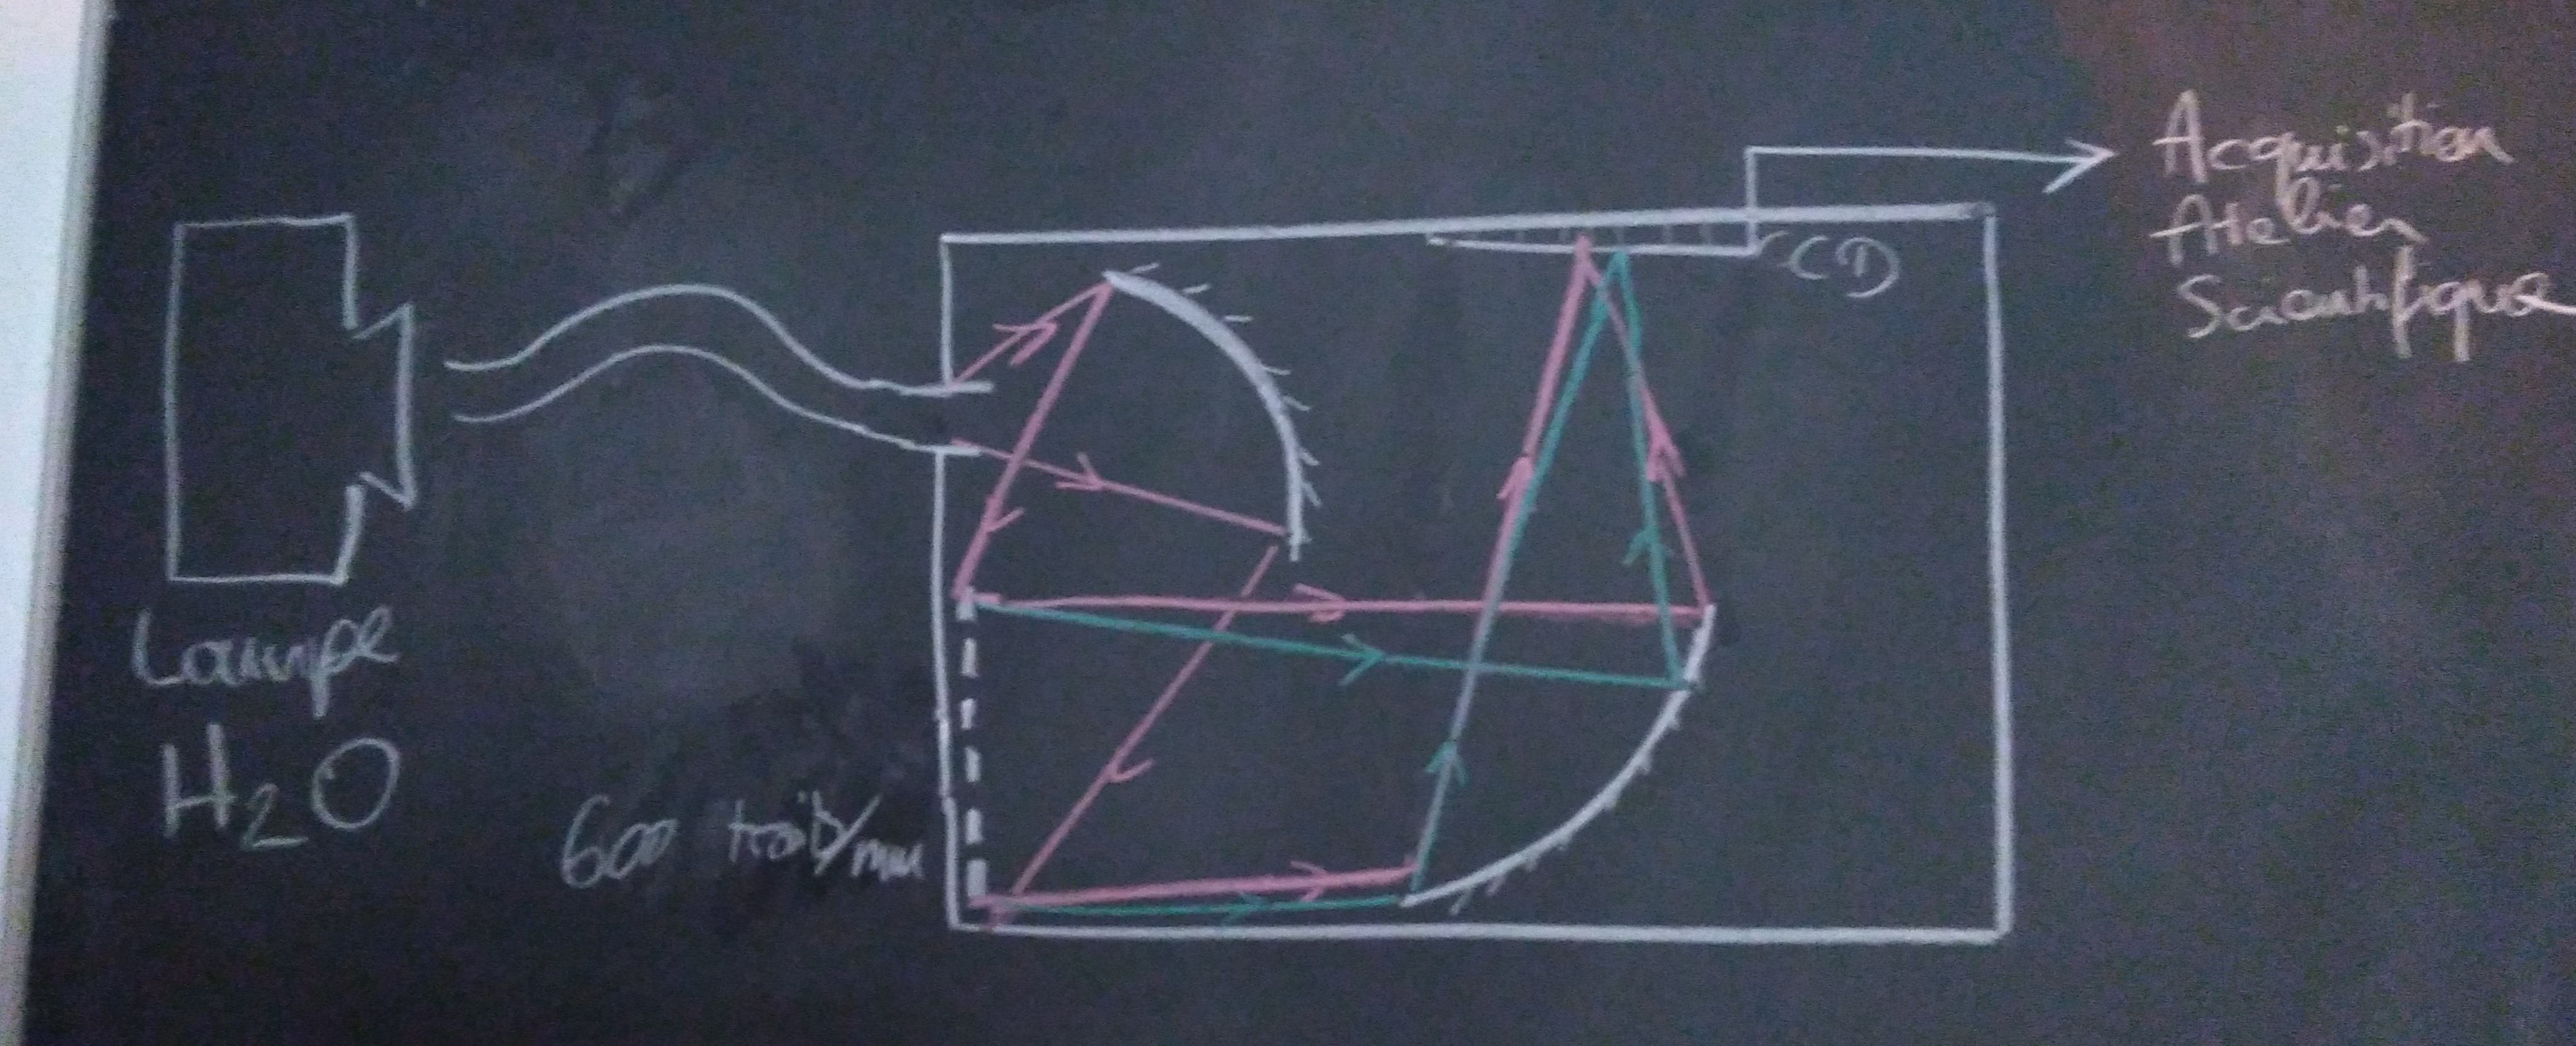
\includegraphics[width=12cm]{spectro}}
\end{figure}

Il est possible d'étalonner le spectromètre en mesurant la position des raies dans le spectre d'un atome bien connu, comme en général l'hydrogène ou l'hélium. On mesure la position des raies en prenant le max d'intensité $I_m$, et en prenant les position des deux points à $I_m/2$, on évalue alors la position de la raie en prenant la moyenne de ces deux mesures.  On trace alors $\lambda_{spectro}(\lambda_{tab})$ et on vérifie si on a bien une droite de coefficient directeur égal à 1, ce qui signifie alors que l'on a un spectromètre étalonné.\\

On peut alors regarder si le modèle de Bohr décrit bien la réalité en prenant les raies visibles de l'hydrogène produit par une lampe à eau (série de Balmer) et regarder si cela correspond avec la formule de Rydberg 
\begin{eqnarray}
\frac{1}{\lambda_{nm}} = R_y\left(\frac{1}{n^2}-\frac{1}{m^2}\right)
\end{eqnarray}
avec $n=2$ pour la série de Balmer, et $R_y = $. On relève la position des raies avec le même protocole que pour l'étalonnage, et puis on trace $\frac{1}{\lambda_m}(1/m^2)$. On peut alors, avec la modélisation adaptée, voir si on retrouve la valeur de $R_y$ et de $n$ prédites par notre modèle, ce qui permet de le valider ou non.\\

On peut maintenant regarder si notre spectromètre permet de résoudre ou non le doublet du sodium, on constate alors que l'on ne peut distinguer qu'une raie, plus large certes et qui permet donc de deviner que c'est peut être un doublet, mais qui ne permet pas de conclure. On va donc maintenant explorer d'autres techniques de spectrométrie afin de voir si elles permettent de résoudre ce doublet.

\section{Le goniomètre}

\begin{figure}
	\centerline{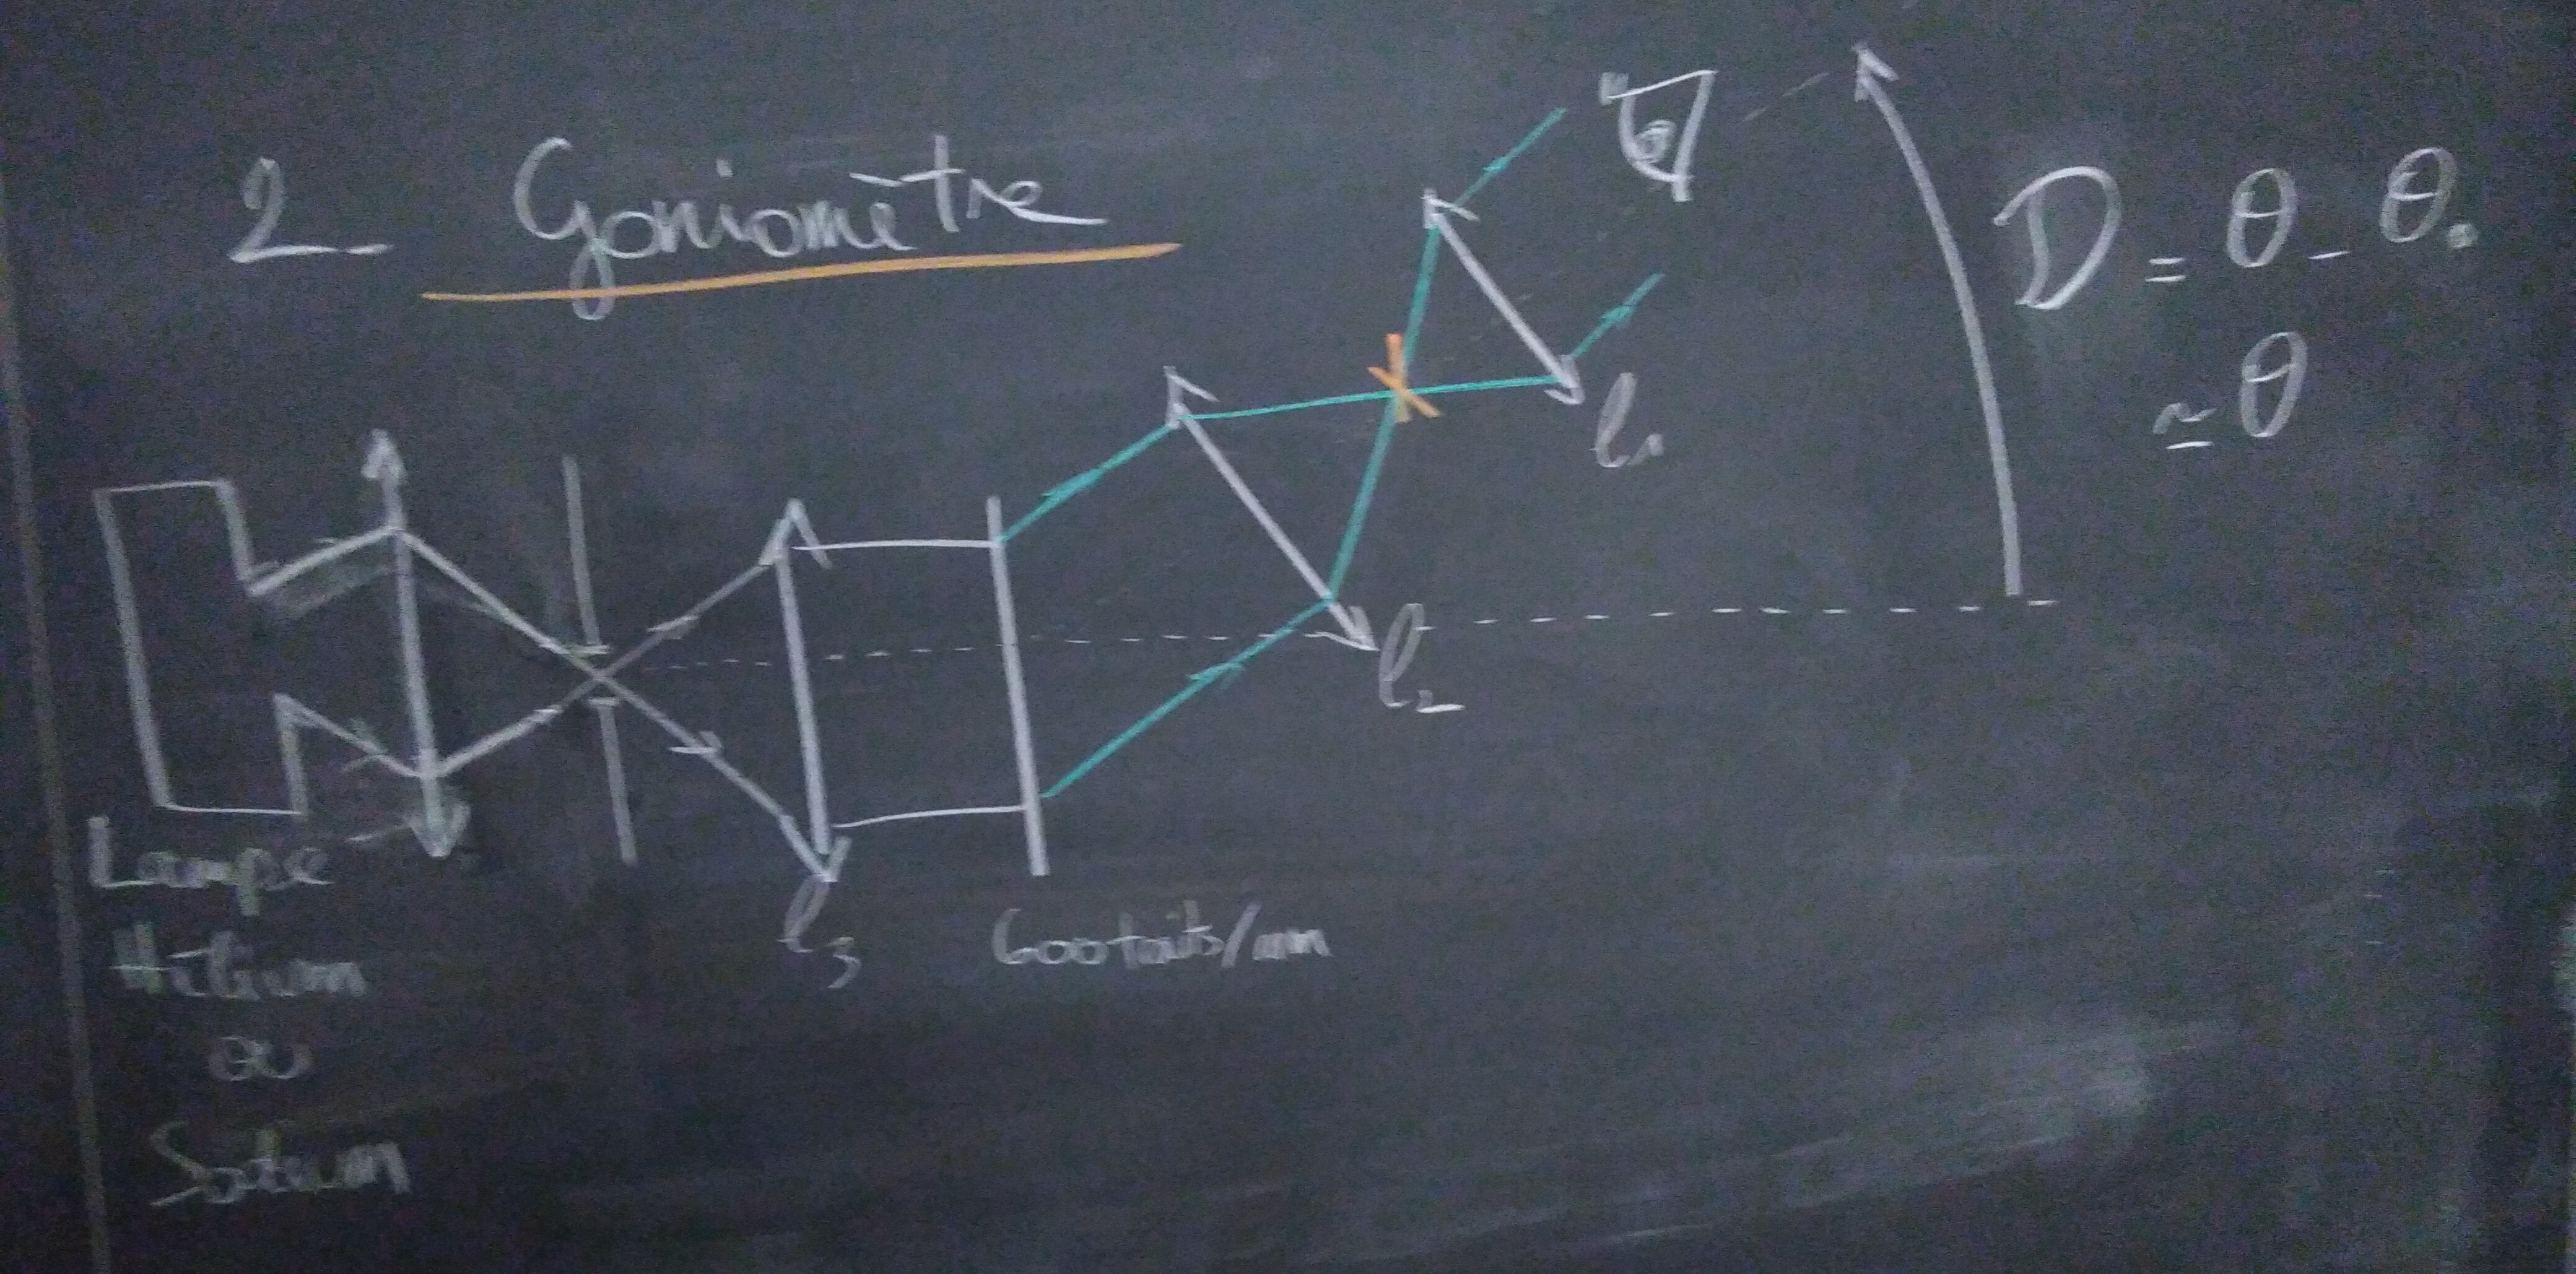
\includegraphics[width=12cm]{gonio}}
\end{figure}

Réglages de l'appareil :
\begin{itemize}
	\item On commence par faire la mise au point de la lentille de sortie de l'oculaire sur le réticule (croix noire). 
	\item On utilise ensuite un miroir ou les 4\% de réflexion du réseau pour acollimater la lentille d'entrée de l'oculaire (il faut d'abord "activer" la lumière avec un petit interrupteur sur l'oculaire). Le but est que l'oculaire forme les images qui sont à l'infini dans le plan contenant le réticule (ainsi on verra les raies et le réticule nettes en même temps, ce qui permet de pointer la position angulaire des raies en les superposant).
	\item Enfin on règle la lentille devant la fente afin d'avoir (en sortie de l'oculaire) une image nette de la fente.
	\item Si on veut travailler en incidence normale il faut tout d'abord aligner l'oculaire et la fente+lentille en utilisant l'ordre 0, on fixe alors la position de l'oculaire. Ensuite on accolimate avec le réseau : on superpose le réticule et l'image de sa réflection sur le réseau en jouant sur les molettes du plateau soutenant le réseau. On a alors que le plan du réseau est orthogonal à l'axe oculaire - fente.
\end{itemize}

Attention il faut repérer la position du zéro, qui n'est pas à la graduation 0, on mesurera donc la position des raies relativement à ce zéro.\\

Pour utiliser la relation des réseaux 
\begin{eqnarray}
a(\sin\theta - \sin\theta_0) = p\lambda
\end{eqnarray}
avec p un entier, $a$ le pas du réseau, $\theta_0$ l'angle d'incidence que fait le rayon provenant de la fente avec la normale au réseau, et $\theta$ la position angulaire de la raie en question par rapport à la normale du réseau, il faudra veiller à mettre les décimales de $\theta$ en 100e de ° et non en minute d'angle.

\subsection{Étalonnage}
Pour vérifier la qualité de notre réglage on peut prendre un spectre connu comme celui de l'hélium, pointer les raies au premier ordre et tracer 
\begin{eqnarray}
\lambda_n^{tab}(\sin\theta_n)
\end{eqnarray}
On modélise ensuite par une droite, qui doit alors avoir une ordonée à l'origine compatible avec 0, et un coefficient directeur compatible avec $a$ le pas du réseau si l'on est bien en incidence normale.

\subsection{Évaluation de $\Delta\lambda$ pour le doublet du sodium}
On a, la dispersion angulaire qui est définie, dans le cas $\theta_0=0$ (c'est à dire $\theta=D$) comme 
\begin{eqnarray}
\mathcal{D}_a = \frac{dD}{d\lambda} = \frac{p}{a\cos D}
\end{eqnarray}

On mesure $\theta_{D1} = 259,533^o$ et $\theta_{D2} = 269,475^o$, avec une incertitude de $1/\sqrt{6}$ minute d'angle, ce qui correspond à un écart angulaire $\Delta \theta = 3,5' = 0.058^o$ entre les deux raies du doublet du sodium à l'ordre 2, cela mène à 
\begin{eqnarray}
\Delta \lambda = \frac{\Delta \theta}{\mathcal{D}_a} = \frac{a \cos D \Delta \theta}{2} \simeq 0.5899\;nm 
\end{eqnarray}
avec $\theta_D \simeq 45,5^o$, et avec l'incertitude 
\begin{eqnarray}
\left(\frac{u(\Delta\lambda)}{\Delta \lambda}\right)^2 = \left(\frac{u(\Delta\theta)}{\Delta \theta}\right)^2 + \sin^2\theta_D\left(\frac{u(\theta_D)}{\theta_D}\right)^2 \simeq \left(\frac{u(\Delta\theta)}{\Delta \theta}\right)^2 \simeq0.00014\;\Rightarrow u(\Delta\lambda) = 0.1\;nm
\end{eqnarray}
où $\Delta \theta = \sqrt{2}/\sqrt{6}'=0.0095^o$. On a donc finalement 
\begin{equation}
\Delta \lambda = 0.6 \pm 0.1 \;nm
\end{equation}
on voit ici que bien que l'on arrive à résoudre le doublet, on a une précision assez médiocre puisque notre incertitude relative est de l'ordre de la dizaine de pour cent. On peut utiliser un système différent : l'interféromètre de Michelson, pour résoudre ce doublet avec une meilleure précision.

\section{Spectrométrie interférentielle}
On va résoudre le doublet du sodium à l'aide d'un interféromètre de Michelson réglé en lames parallèles. On a comme visibilité
\begin{eqnarray}
V(\delta) = \cos\left(\frac{\pi\delta \Delta\lambda}{\lambda_0^2}\right)
\end{eqnarray}
avec $\frac{\delta}{2}$ l'écart (en terme de différence de marche) entre les deux miroirs.\\
Là encore on repère les positions $x_n$ des annulations de contraste, en regardant la position $x_n^1$  où on commence à perdre le contraste et $x_n^2$ où le contraste réapparait, et en prenant donc $x_n = \frac{x_n^1+x_n^2}{2}$. On trace alors $x_n(n)$ avant de modéliser par une droite pour obtenir un coefficient directeur $\Delta x$. On a alors 
\begin{eqnarray}
\Delta \lambda = \frac{\lambda_0^2}{2\Delta x}
\end{eqnarray}

Pour ce qui est de l'incertitude on a, avec le mode opératoire choisi, $\sigma_n = \frac{x_n^2-x_n^1}{\sqrt{6} }$ (distribution triangulaire). L'incertitude finale $u(\Delta x)$ est alors donnée par la régression effectuée par régressi, et on peut prendre pour $\lambda_0$ la valeur tabulé, d'incertitude relative négligeable, ou bien utiliser la valeur obtenue avec le goniomètre dont on connait l'incertitude associée.\\
On trouve alors un résultat avec une précision cette fois à quelques 100e de nm.

\section*{Questions}
Pour la troisième partie, le point ajouté en direct étant en dehors de la courbe, faut il le supprimer pour modéliser ?\\
Oui car il pollue le résultat obtenu et les incertitudes associées.\\

Quelle est la définition de pouvoir de résolution ?\\ 
Le pouvoir de résolution décrit la capacité à distinguer deux raies, il s'exprime comme $\Delta\lambda/\lambda$. Il vaut 600 pour le spectro USB, et ici 25mm$\times$600 traits/mm = 15000 pour le gonio.\\

Comment estimer là de manière pratique le PR du gonio ?\\
on distingues deux raies séparées d'environ 0.6nm, et qui font environ 0.1nm de large on a donc PR $\simeq 600/0.1 = 6000$ puisqu'on regarde des raies à environ 600nm.\\

Et pour le spectro USB ?\\
On a une épaisseur apparente des raies de 0.8nm et donc un PR de 600/0.8 = 750.\\

Et pour le michelson ?\\
On a 
\begin{eqnarray}
\delta \lambda = \frac{\lambda_0^2}{2L} = \frac{(6.10^{-7})^2}{2\times 6.10^{-2}} =  3.10^{-12}
\end{eqnarray}
avec L la longueur maximale sur laquelle on peut charioter, on a donc un PR de $6.10^7/3.10^{-12}=2.10^5$.

\section*{Remarques}
Pour chaque manip il faut expliciter le pouvoir de résolution à la fin de chaque partie.\\
Pour Rydberg modéliser directement avec la forme théorique, comme ça on a directement les coefficients avec leurs incertitudes : on gagne du temps.


\end{document}